\section{Threat Model and Security Objectives}
\label{sec:threat_model}

To rigorously evaluate the Virtual Private Phone architecture, we define our threat model based on realistic adversarial capabilities, operational trust boundaries, and formalized security goals.

\subsection{Adversary Profiles and Capabilities}
We classify adversaries into four distinct tiers based on resource availability, physical access, and forensic sophistication:

\subsubsection{$\mathcal{A}_1$: The State/Forensic Adversary (Law Enforcement / Border Inspection)}
\begin{itemize}
    \item \textbf{Capabilities:} The adversary obtains immediate physical custody of the frontend handset. The device may be seized in an active, unlocked (AFU) state or locked with a known or coerced biometric/PIN. The adversary possesses state-of-the-art digital forensics hardware (e.g., Cellebrite Premium, Magnet GrayKey) capable of bootloader exploitation, direct memory access (DMA), and chip-off analysis.
    \item \textbf{Tactics:} Immediate insertion into an RF-shielded Faraday enclosure to prevent remote wipe; memory acquisition via cold-boot or JTAG testing; persistent storage imaging; extraction of application SQLite databases and keychain stores.
    \item \textbf{Constraints:} The adversary does not have physical access to the operator's private residence where the backend core is located, nor do they possess the out-of-band cryptographic credentials required for backend authentication.
\end{itemize}

\subsubsection{$\mathcal{A}_2$: The Opportunistic / Street-Level Adversary}
\begin{itemize}
    \item \textbf{Capabilities:} Gains physical possession of the handset via opportunistic theft (e.g., snatch-and-grab on public transit). 
    \item \textbf{Tactics:} Attempts to access mobile banking applications, exploit SMS 2FA tokens arriving on the device, or perform a factory reset for secondary hardware resale.
    \item \textbf{Constraints:} Lacks zero-day exploit capabilities or specialized forensic laboratory infrastructure.
\end{itemize}

\subsubsection{$\mathcal{A}_3$: The Network Intermediary (IMSI Catchers / Rogue APs)}
\begin{itemize}
    \item \textbf{Capabilities:} Deploys cell-site simulators (StingRays)~\cite{vandenbroek2015imsi}, compromised public Wi-Fi hotspots, or conducts SS7/Diameter signaling attacks at the carrier level.
    \item \textbf{Tactics:} Interception of unencrypted transit packets, metadata harvesting, man-in-the-middle (MitM) TLS stripping, and cellular location tracking.
    \item \textbf{Constraints:} Cannot break standardized modern cryptographic primitives (e.g., Curve25519, ChaCha20-Poly1305, AES-256-GCM).
\end{itemize}

\subsubsection{$\mathcal{A}_4$: The Advanced Persistent Threat (Mercenary Spyware)}
\begin{itemize}
    \item \textbf{Capabilities:} Possesses zero-click mobile exploits (e.g., NSO Group's Pegasus / FORCEDENTRY~\cite{marczak2021pegasus}) delivered via iMessage, WhatsApp, or baseband vulnerability chains.
    \item \textbf{Tactics:} Kernel-level compromise of the device OS, persistent rootkit installation, covert activation of microphones and cameras, exfiltration of stored credentials.
    \item \textbf{Constraints:} Restricted to exploiting the software surface exposed by the device.
\end{itemize}

\subsection{Trust Boundaries and Assumptions}
The VPP establishes a strict architectural boundary dividing the operational domain into two distinct zones:

\begin{figure}[h!]
\centering
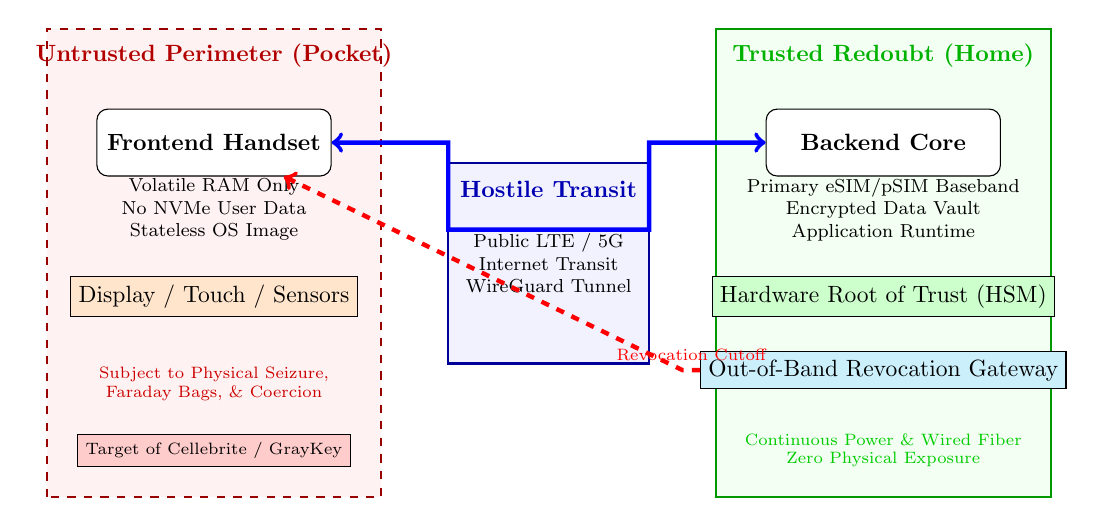
\begin{tikzpicture}[scale=0.85, every node/.style={transform shape}]
    % Untrusted Domain
    \draw[red!60!black, dashed, thick, fill=red!5] (-0.5,-3.5) rectangle (4.5,3.5);
    \node[red!70!black, font=\bfseries] at (2,3.1) {Untrusted Perimeter (Pocket)};
    
    \node[draw, rectangle, rounded corners, fill=white, minimum width=3.5cm, minimum height=1cm] (handset) at (2,1.8) {\textbf{Frontend Handset}};
    \node[font=\footnotesize, align=center] at (2,0.8) {Volatile RAM Only\\No NVMe User Data\\Stateless OS Image};
    \node[draw, rectangle, fill=orange!20, minimum width=3.5cm] (sensors) at (2,-0.5) {Display / Touch / Sensors};
    \node[font=\scriptsize, red!80!black, align=center] at (2,-1.8) {Subject to Physical Seizure,\\Faraday Bags, \& Coercion};
    \node[draw, rectangle, fill=red!20, font=\scriptsize] at (2,-2.8) {Target of Cellebrite / GrayKey};

    % Network Domain
    \draw[blue!60!black, thick, fill=blue!5] (5.5,-1.5) rectangle (8.5,1.5);
    \node[blue!70!black, font=\bfseries] at (7,1.1) {Hostile Transit};
    \node[align=center, font=\footnotesize] at (7,0) {Public LTE / 5G\\Internet Transit\\WireGuard Tunnel};

    % Trusted Domain
    \draw[green!60!black, thick, fill=green!5] (9.5,-3.5) rectangle (14.5,3.5);
    \node[green!70!black, font=\bfseries] at (12,3.1) {Trusted Redoubt (Home)};
    
    \node[draw, rectangle, rounded corners, fill=white, minimum width=3.5cm, minimum height=1cm] (backend) at (12,1.8) {\textbf{Backend Core}};
    \node[font=\footnotesize, align=center] at (12,0.8) {Primary eSIM/pSIM Baseband\\Encrypted Data Vault\\Application Runtime};
    \node[draw, rectangle, fill=green!20, minimum width=3.5cm] (hsm) at (12,-0.5) {Hardware Root of Trust (HSM)};
    \node[draw, rectangle, fill=cyan!20, minimum width=3.5cm] (oob) at (12,-1.6) {Out-of-Band Revocation Gateway};
    \node[font=\scriptsize, green!80!black, align=center] at (12,-2.8) {Continuous Power \& Wired Fiber\\Zero Physical Exposure};

    % Connections
    \draw[<->, ultra thick, blue] (handset) -- (5.5,1.8) -- (5.5,0.5) -- (8.5,0.5) -- (8.5,1.8) -- (backend);
    \draw[->, ultra thick, dashed, red] (oob) -- ++(-3,0) node[midway, above, font=\scriptsize] {Revocation Cutoff} -- (handset);
\end{tikzpicture}
\caption{Architectural trust boundaries of the Virtual Private Phone.}
\label{fig:trust_boundaries}
\end{figure}

\begin{enumerate}
    \item \textbf{The Backend Core is Physically Secure:} Located within a private domestic redoubt with uninterrupted power, high-bandwidth optical fiber connection, and physical perimeter controls. Physical intrusion into this facility requires search warrants and kinetic entry, a separate legal and operational barrier.
    \item \textbf{The Frontend Handset is Expendable and Untrusted:} The pocket device is assumed to be vulnerable to loss, seizure, and surveillance. We treat the frontend as a Byzantine entity once physical custody is lost.
    \item \textbf{Network Transport is Hostile:} All communication between nodes traverses untrusted public cellular networks, routing through commercial ISPs and potentially monitored transit paths.
\end{enumerate}

\subsection{Formal Security Objectives}
The VPP system must guarantee the following fundamental security properties:

\begin{property}[Confidentiality Under Confiscation]
Let $\mathcal{D}_{core}$ denote the persistent datastore of the user, and $\mathcal{D}_{handset}$ denote the extractable persistent data on the frontend handset. The system guarantees that:
\begin{equation}
    |\mathcal{D}_{handset}| = 0 \quad \text{and} \quad I(\mathcal{D}_{handset}; \mathcal{D}_{core}) = 0
\end{equation}
where $I(X; Y)$ denotes mutual information. Physical possession of the frontend reveals zero bits of historical application databases, private encryption keys, or archived media.
\end{property}

\begin{property}[Revocation Finality and Instantaneous Severance]
Upon receipt of an authenticated out-of-band revocation signal $S_{rev}$ by the backend core at timestamp $t_{rev}$, the backend terminates the cryptographic session keys $K_{session}$. For all subsequent requests $R_t$ with $t > t_{rev}$:
\begin{equation}
    P(\text{Accept}(R_t) \mid S_{rev}) = 0
\end{equation}
Even if an adversary holds an unlocked frontend in their hand, subsequent screen taps or network requests fail deterministically.
\end{property}

\begin{property}[Volatile Memory Zeroization]
Upon local session termination, network timeout, or duress signal, all volatile buffers allocated to video decoding, framebuffer storage, and session keys are wiped using cryptographically secure zeroization primitives ($\texttt{explicit\_bzero}$ / memory barriers), defeating cold-boot and DMA memory extraction attacks~\cite{halderman2008coldboot}.
\end{property}
